\documentclass[11pt]{article}
\usepackage[margin=0.75in]{geometry}            % See geometry.pdf to learn the layout options. There are lots.
\geometry{letterpaper}                                  % ... or a4paper or a5paper or ... 
%\geometry{landscape}                           % Activate for rotated page geometry
%\usepackage[parfill]{parskip}                  % Activate to begin paragraphs with an empty line rather than an indent
\usepackage{graphicx}                           % Use pdf, png, jpg, or eps§ with pdflatex; use eps in DVI mode
                                                                % TeX will automatically convert eps --> pdf in pdflatex                
\usepackage{amssymb}
\usepackage{upquote}
\usepackage{amsmath}
\usepackage{multicol}
\usepackage{subcaption}
\usepackage{wrapfig}
\usepackage{float}

%-----------------------------------------------------------------------------
% Special-purpose color definitions (dark enough to print OK in black and white)
\usepackage{color}
% A few colors to replace the defaults for certain link types
\definecolor{orange}{cmyk}{0,0.4,0.8,0.2}
\definecolor{darkorange}{rgb}{.71,0.21,0.01}
\definecolor{darkgreen}{rgb}{.12,.54,.11}
%-----------------------------------------------------------------------------
% The hyperref package gives us a pdf with properly built
% internal navigation ('pdf bookmarks' for the table of contents,
% internal cross-reference links, web links for URLs, etc.)
\usepackage{hyperref}
\hypersetup{pdftex, % needed for pdflatex
  breaklinks=true, % so long urls are correctly broken across lines
  colorlinks=true,
  urlcolor=blue,
  linkcolor=darkorange,
  citecolor=darkgreen,
}


\title{Finance Project\\
  Stat 222, Spring 2016}

\author{
  Siyao Chang, Mengfei Jiang, Tianyi Zhang\\
  \texttt{your github account}
}


\begin{document}
\maketitle

\abstract{This paper studies the performance of a variety of machine learning techniques in classifying the mid-price changes and price spread crossings from the high-frequency limit order book of Apple Inc (AAPL) on a trading day. The idea of feature selection and model building originates from the 2014 paper by Kercheval and Zhang~\cite{financesvm}. In addition to the ordinary data processing, model fitting and assessment, this paper also interprets the fitted model, and tries to implement the trading strategies in the model to compute the ideal profit.}


\section{Introduction}
The modern computing systems enables the high-frequency trading in stock markets. From Kercheval and Zhang's paper in 2014~\cite{financesvm}, high frequency trading accounted for 84\% total stock trades, and thus utilizing data from limit order book becomes crucial to capture the dynamics of stock markets. The purpose of this paper is to build classification models to help the buy/sell decision for the AAPL stock from the limit order book containing different levels of bid and ask prices information.\\
From Kercheval and Zhang in 2014~\cite{financesvm}, the features are grouped in the basic set, the time-insensitive set, and the time-sensitive set. We built up the classification models based on the subset of these 3 sets. The basic set contains the 10 levels of bid and ask prices and volumes. The time-insensitive set contains the mid-prices and bid-ask spreads, price differences, mean prices and volumes, accumulated differences for 10 different levels. Considering the computational complexity, we only use the price and volume derivatives from the time-sensitive set. The reponse variables we have considered in this paper are a factor variable of mid-price changes and another factor variable of spread-crossings. Each of the response variable could fall in three classes: upward(U), downward(D), stationary(S).\\
The paper first clarifies the data preprocessing, then addresses the model fitting and assessment. After finalizing the models, a section followed will talk about how to interpret models and how models matches common financial knowledge. Finally, there will be a section talking about the implementation of the trading strategies from the model, where profit will be computed.
\section{Data Preprocessing}
The data we used is obtained from the limit order book of the SPY index. The specific stock we are interested in is the APPLE stock. Our data include the prices and volumes of AAPL from 9:30AM to 12:28PM on May 22, 2012 for 10 levels of bid and ask for each time-stamped event. \\
Since we are trying to predict whether the stock price has an upward, stationary or downward trend, we need to create these labels first. We created the labels in two ways: 1) using the mid-price movement and 2) using the bid-ask spread crossing. \\
The mid-price is the mean of the best ask price and best bid price, in our case, the level 1 ask and bid price. It is calculated as $P_t^{mid} = \frac{1}{2}(P_t^{ask} + P_t^{bid})$. We compare the mid-price of the current time point to the mid-price at $\Delta t$ later timestamp. If the later mid-price is larger than the current mid-price plus tick-size, then the stock has an upward trend. Similarly, we get a downward trend if the later mid-price is smaller than the current mid-price minus tick-size and stationary trend otherwise. We use these three possible outcomes of mid-price movements (upward, stationary and downward) as our class labels. \\
Bid-ask spread crossing is a more common way in real market when determining trends. We can also determine the three types of trends with spread crossing. There is an upward price spread crossing when the best bid price at a certain later timestamp exceeds the best ask price at the current timestamp ($P_{t+\Delta t}^{bid} > P_t^{ask}$). Similarly, when the best ask price at a later timestamp is less than the best bid price at the current timestamp, we have a downward trends. In all other situations (i.e. $P^{ask}_{t+\Delta t} > P^{bid}_t$ and $P^{bid}_{t+\Delta t} < P^{ask}_t$), we have a stationary trend. In this project, we use both ways to create label classes and train models. \\
Now, we pre-process our raw data into suitable and meaningful predictors. All the features and their corresponding descriptions are shown in Table 1, divided into three categories: basic, time-insensitive and time-sensitive. First, we extract the ask and bid price, as well as the ask and bid volume (collectively defined as $v_1$) for each of the 10 levels from the raw dataset to form our basic feature set. \\
Our time insensitive set includes features $v_2, v_3, v_4, v_5$. These features are bid-ask spreads and mid-prices ($v_2$), price difference ($v_3$), mean prices and volumes ($v_4$) and accumulated differences ($v_5$) respectively. We wrote functions to calculate each feature. \\
In the time-sensitive set, we have features $v_6, v_7, v_8, v_9$. $v_6$ is the average time derivative of price and volume, computed over a specified $\Delta t$. Again, we wrote a function, taking $\Delta t$ as an input to calculate the price and volume derivatives. $v_7, v_8, v_9$ focuses on the intensity and acceleration of the different trading types (limit, market and cancellation). $v_7$ is the average intensity of each type; $v_8$ is the relative intensity indicators; $v_9$ is the accelerations of market and limit order bids and asks. Features $v_7, v_8, v_9$ require the use of the message book dataset and is computationally exhaustive. Therefore, we left them out and only used features $v_1 - v_6$ when training our models.

\begin{center}
\renewcommand{\arraystretch}{1.4}
\begin{tabular}[2pt]{|l|l|}
\hline
Basic Set & Description($i$ = LOB level)\\
\hline
$v_1 = \{P_i^{ask}, V_i^{ask}, P_i^{bid}, V_i^{bid}\} $ & price and volume (10 levels) \\
\hline
\multicolumn{2}{c} {} \\
\hline
Time-insensitive Set & Description($i$ = LOB level)\\
\hline
$v_2 = \{P_i^{ask}-P_i^{bid}, (P_i^{ask}+P_i^{bid})/2\} $ & bid-ask spreads and mid-prices \\
$v_3 = \{P_{10}^{ask}-P_1^{ask}, P_{1}^{bid}-P_{10}^{bid}, |P_{i+1}^{ask}-P_i^{ask}|, |P_{i+1}^{bid}-P_{i}^{bid}\} $ & price differences (10 levels) \\
$v_4 = \{\frac{1}{n}\sum_{i=1}^{n}P_i^{ask}, \frac{1}{n}\sum_{i=1}^{n}P_i^{bid}, \frac{1}{n}\sum_{i=1}^{n}V_i^{ask}, \frac{1}{n}\sum_{i=1}^{n}V_i^{bid}\} $ & mean prices and volumes \\
$v_5 = \{\sum_{i=1}^{n}(P_i^{ask}-P_i^{bid}), \sum_{i=1}^{n}(V_i^{ask}-V_i^{bid})\} $ & accumulated differences \\
\hline
\multicolumn{2}{c} {} \\
\hline
Time-sensitive Set & Description($i$ = LOB level)\\
\hline
$v_6 = \{dP_i^{ask}, dV_i^{ask}, dP_i^{bid}, dV_i^{bid}\} $ & price and volume derivatives \\
%$v_7 = \{\lambda_{\Delta t}^{la}, \lambda_{\Delta t}^{lb}, \lambda_{\Delta t}^{ma}, \lambda_{\Delta t}^{mb}, \lambda_{\Delta t}^{ca}, \lambda_{\Delta t}^{cb}\} $ & average intensity of each type \\
%$v_8 = \{\textbf{1}_{\{\lambda_{\Delta t}^{la}>\lambda_{\Delta T}^{la}\}}, \textbf{1}_{\{\lambda_{\Delta t}^{lb}>\lambda_{\Delta T}^{lb}\}}, \textbf{1}_{\{\lambda_{\Delta t}^{ma}>\lambda_{\Delta T}^{ma}\}}, \textbf{1}_{\{\lambda_{\Delta t}^{mb}>\lambda_{\Delta T}^{mb}\}}\} $ & relative intensity indicators \\
%$v_9 = \{d\lambda^{ma}, d\lambda^{lb}, d\lambda^{mb}, d\lambda^{la}\} $ & accelerations (market/limit) \\
\hline
\end{tabular}

\vspace{0.5 cm}
\small \textbf{Table 1}: Feature vector set (basic, time-insensitive and time-sensitive set) for 10 levels of LOB
\end{center}
%\normalsize
After transforming the dataframe to the feature space, we divide the dataset into two parts, one from 9:30AM to 11:00AM (called set1 in future text), where we will use in the model fitting, and the other from 11:00AM to 12:00PM (called set2 in future text), where we use it to implement the trading strategies.

\section{Model Fitting}
To classify the mid-price movements and the bid-ask spread crossings, we have used the Support Vector Machine (SVM) with radial basis function kernel (RBF) and the Random Forest. Firstly, we randomly divide the set1 into three parts: training set (50\%), validation set (25\%), and test set (25\%). We will use the training set to train the machine learning models, and use the validation set to tune the model parameters (such as the regularization parameter in SVM, $\Delta t$, and the tick-size defining the stationarity for mid-price movements). In the future model fitting, we have carefully chose $\Delta t$ to be 30 events for simplicity, because calculating actual time could be computational expensive, as there could be multiple events in the exact same second. Choosing a small $\Delta t$ would cause the stationary class to dominate, which cause an imbalanced classification problem, and a large $\Delta t$ would make prediction harder.  Both of SVM and Random Forest alogrithms were applied by the scikit-learn library in python.\\
Notice that when tuning model parameters, we have used the F-1 meausre on the \textbf{validation set} to be the error criterion. The F-1 measure would also be used later in the model assessment on the test dataset:
\begin{align*}
precision=\frac{\#\ correctly\ labeled\ certain\ class}{\#\ certain\ class\ in\ predictions}\\
recall=\frac{\#\ correctly\ labeled\ certain\ class}{\# certain\ class\ in\ sample}\\
F1=\frac{2*precision*recall}{precision+recall}
\end{align*}
\subsection{Mid-Price Movement Based Model Fitting}
First of all we had to choose an appropriate tick-size to define stationary when labeling the mid-price movement. If we defined the tick-size to be zero, then there could be no stationary data points because mid-prices at two time points were rarely exactly the same. On the other hand, to aviod the imbalanced data classification problem, it would be better to make each class distributing roughly evenly. We chose the tick-size to be 0.01, where we defined stationary in the range $[midprice-0.01,midprice+0.01]$
\subsubsection{SVM}
In SVM, the parameter we tuned was the inverse regularization parameter C. A smaller C value corresponds to a softer margin, allowing more misclassification of training data points to prevent overfitting. Figure~\ref{fig:mid_f1} showed the F-1 measures on the training and the validation sets at different C levels. The eventual model was trained on 10,000 samples by oversampling from the combined set of the training and the validation (i.e. 75\% of the data in set1), and we set the C to be the optimal value of 10.
\begin{figure}[H]
\centering
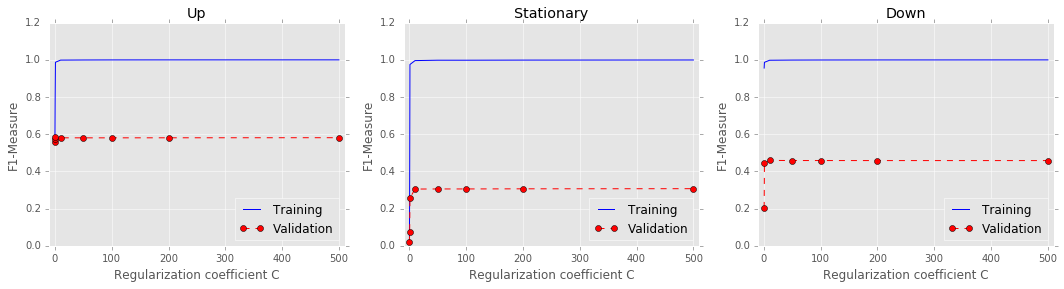
\includegraphics [width=0.9\linewidth,height=0.22\linewidth]{./figures/svm_mid_f1.png}
\caption{F-1 measure on training and validation sets v.s. regularization coefficient}
\label{fig:mid_f1}
\end{figure}
\subsubsection{Random Forest}
\begin{figure}[H]
\centering
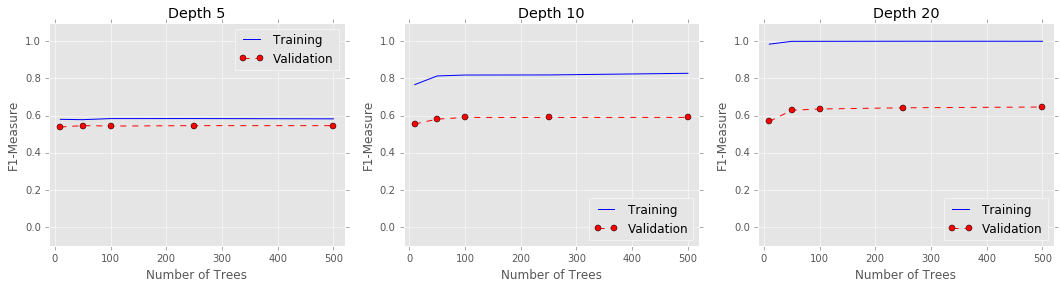
\includegraphics [width=0.9\linewidth,height=0.22\linewidth]{./figures/tree_mid_up_f1.png}
\caption{F-1 measure for Up on training and validation sets v.s. max depth and number of trees}
\label{fig:mid_f1_1}
\end{figure}
\begin{figure}[H]
\centering
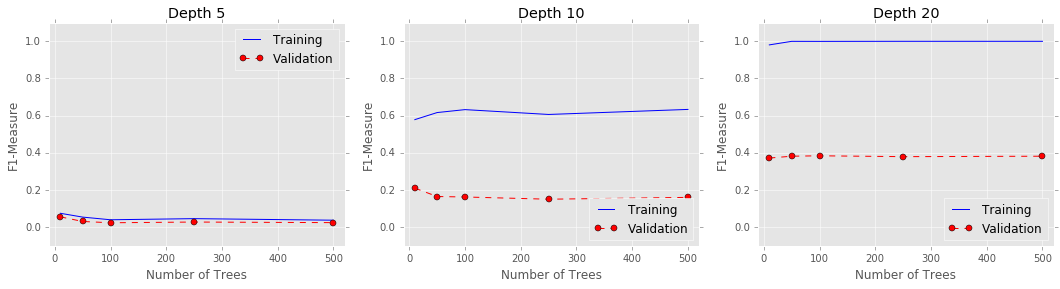
\includegraphics [width=0.9\linewidth,height=0.22\linewidth]{./figures/tree_mid_stat_f1.png}
\caption{F-1 measure for Stationary on training and validation sets v.s. max depth and number of trees}
\label{fig:mid_f1_2}
\end{figure}
\begin{figure}[H]
\centering
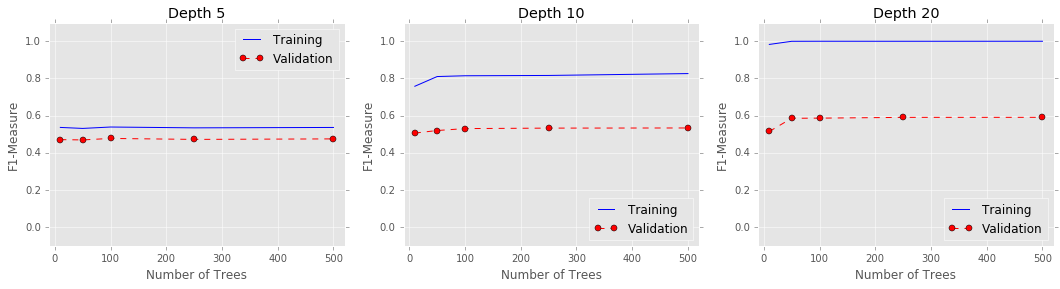
\includegraphics [width=0.9\linewidth,height=0.22\linewidth]{./figures/tree_mid_down_f1.png}
\caption{F-1 measure for Down on training and validation sets v.s. max depth and number of trees}
\label{fig:mid_f1_3}
\end{figure}
In the Random Forest, the parameters we tuned were the number of trees and the maximum depth of each tree, while we set the number of feature candidates for each tree to be the square root of the total feature number by convention. Deeper trees allowed for more splits reducing prediction bias, and averaging over more trees reduced prediction variance. The eventual model was trained on all data points from the combination of the training and the validation (75\% of the set1) with 500 trees of maximum depth of 20. The important features were also extracted for later use as described in subsection~\ref{subsection:economic}.
\subsection{Spread-Crossing Based Model Fitting}
After labeling the spread-crossing for each data point, we found that "stationary" approximately occupied more than 98\% of data points, with the rest being Up or Down. This raised a highly imbalanced data classification problem as pointed in 2005 paper by Chawla~\cite{imbalance}, the model could simply predict all data points to be stationary and gain a 98\% overall accuracy. As it has been pointed in~\cite{imbalance}, we have to oversample the minority classes, or undersample the dominating classes. Considering these sampling strategies, we decided to use ${10\%,80\%,10\%}$ for {Up, Stationary, Down} in the training set. The reason we did not go far away to portions like ${1/3,1/3,1/3}$ was that we did not want to mis-preidict too many stationary data points to Up or Down (which could lead to huge losses when implementing the model).
\subsubsection{SVM}
\begin{figure}[H]
\centering
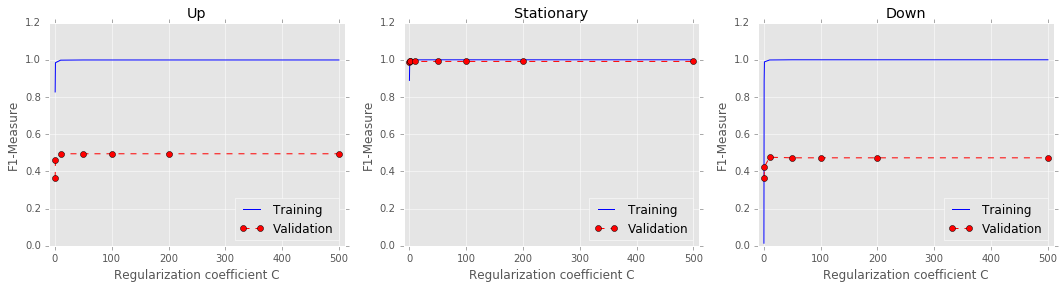
\includegraphics [width=.9\linewidth,height=0.22\linewidth]{./figures/svm_cross_f1.png}
\caption{F-1 measure on training and validation sets v.s. regularization parameter C}
\label{fig:cross_f1}
\end{figure}
We did the similar thing to the SVM in mid-price movement model. Notice that we did not adjust the portion of each class in the validation set, even though we did oversampling in the training set. The eventual model was trained on 10,000 samples by oversampling from the combined set of the training and the validation (i.e. 75\% of the data in Set1), and we set the C to be the optimal value of 10.
\subsubsection{Random Forest}
Parameters were tuned in the same way as in mid-price movement model. The eventual model was trained on resampled data points of the same size as the original, which is the combination of the training and the validation (75\% of the set1). We set the number of trees to be 250 and the max-depth to be 20. Again, the important features were also extracted for later use as described in subsection~\ref{subsection:economic}.
\begin{figure}[H]
\centering
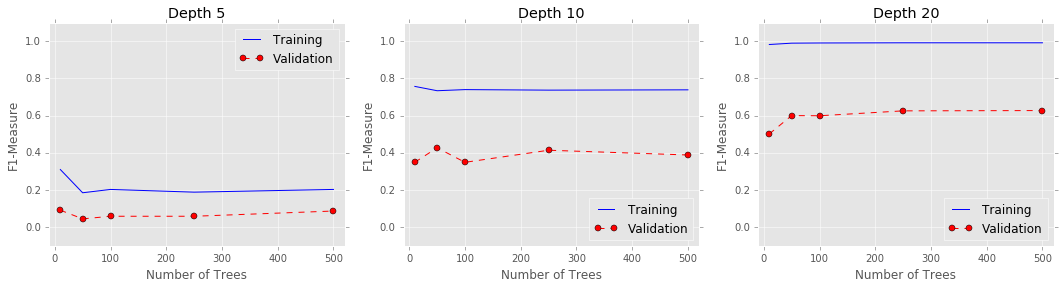
\includegraphics [width=1\linewidth,height=0.25\linewidth]{./figures/tree_spread_up_f1.png}
\caption{F-1 measure for Up on training and validation sets v.s. max depth and number of trees}
\label{fig:spread_f1_1}
\end{figure}
\begin{figure}[H]
\centering
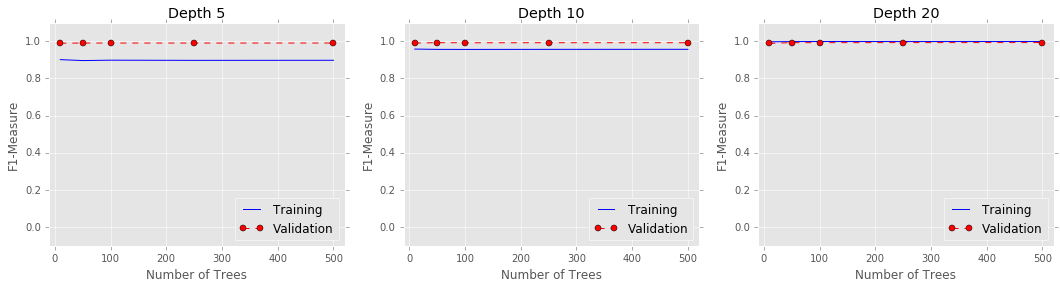
\includegraphics [width=1\linewidth,height=0.25\linewidth]{./figures/tree_spread_stat_f1.png}
\caption{F-1 measure for Stationary on training and validation sets v.s. max depth and number of trees}
\label{fig:spread_f1_2}
\end{figure}
\begin{figure}[H]
\centering
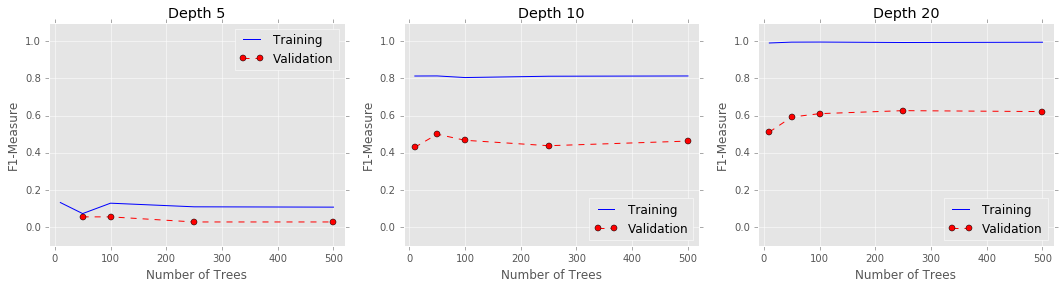
\includegraphics [width=1\linewidth,height=0.25\linewidth]{./figures/tree_spread_down_f1.png}
\caption{F-1 measure for Down on training and validation sets v.s. max depth and number of trees}
\label{fig:spread_f1_3}
\end{figure}


\subsection{Economized Set of Feature Space}
\label{subsection:economic}
In Zhang's 2004 paper~\cite{financesvm}, the authors mentioned the possibility of predicting the price movements by a much smaller subset of the feature space. Considering the frequency of updating models, an economized feature set is desirable for efficiency purposes and saves computational power. Another concern is about the memory use, the entire feature space carried 126 features, which could use a lot memory when analyzing multiple stocks.\\
To get the economized feature set, we used the feature importance index extracted from the random forest in the scikit-learn package. The feature importance measured the contributions of each feature, and it was defined by the reduction in weighted information impurity. With that being said, we first fitted the random forest models over the entire feature space with optimal parameters, and then put top 20 important features shown in \ref{fig:important} with the greatest importance index in the economized feature set. Considering the page limit, we only list top 5 important features for mid-price model and the spread-cross model.\\
Top 5 features for mid-price model:\\
Level 1 Ask Volume, Accumulated Volume Difference, Mean Ask Volume, Mean Bid Volume, and Level 1 Bid-Ask Spread.\\
Top 5 features for spread-cross model:\\
Level 1 Bid-Ask Spread, Level 2 Bid-Ask Spread, Level 3 Bid-Ask Spread, Accumulated Price Difference, and Mean Ask Volume.\\
We then fitted random forests over these two smaller economized feature set, and tuned the parameters using the validation set. The number of trees set for Mid-price model was 250, and the max-depth was 18. The number of trees for the Spread-Cross model was 100, and the max-depth was 18.
\begin{figure}[H]
\centering
\begin{subfigure}{.5\textwidth}
\centering
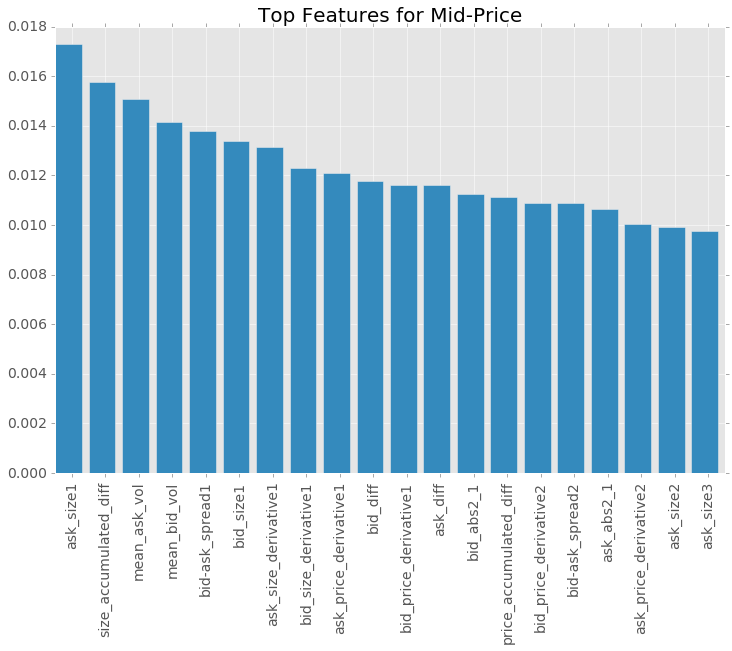
\includegraphics[width=0.95\linewidth,height=0.8\linewidth]{./figures/tree_mid_top_features.png}
\caption{Top features of mid-price models by importance}
\label{fig:mid_important}
\end{subfigure}%
\begin{subfigure}{.5\textwidth}
\centering
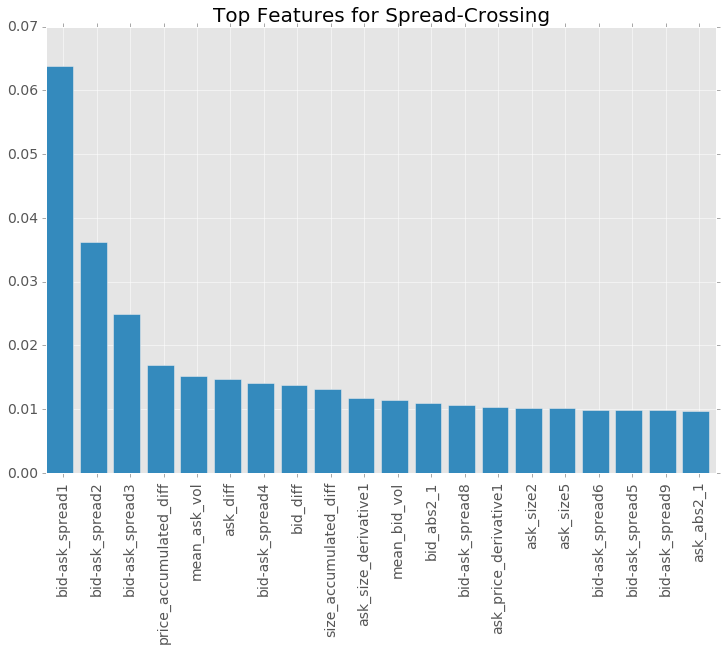
\includegraphics[width=0.95\linewidth,height=0.8\linewidth]{./figures/tree_spread_top_features.png}
\caption{Top features of spread-corss models by importance}
\label{fig:spread_important}
\end{subfigure}
\caption{Economized Set for mid-price and spread-cross models}
\label{fig:important}
\end{figure}


\section{Model Assessment}
To test classification models, performance was measured by three common assessment measures for classification models, which were precision, recall, and F1 measure. The definitons of these measures could be found in the model fitting section.
\subsection{Entire Feature space}
We used the 25\% of the set1 to be the test set, and the result indicates that overall the random forest performed better than SVM with RBF kernels in terms of three common measures, and it took much less time to train a random forest. This also matched the nonlinearity of feature space of LOB, where random forest would perform much better. We also observed that the F-1 measure for Mid-price models was better than Spread-Cross Models. Both of three measures and confusion matrices for four models (mid-price svm, mid-price RF, spread-cross svm, spread-cross RF) are shown below, notice that those models are trained in the entire feature space:
\begin{multicols}{2}
\begin{center}
\renewcommand{\arraystretch}{1.4}
\resizebox{0.8\linewidth}{!}{
\begin{tabular}[2pt]{|c|c|c|c|}
\hline
Label & Precision & Recall & F1-Measure \\
\hline
U & 79.5127\% & 46.2081\% & 58.4490\% \\
S & 22.1084\% & 57.1603\% & 31.8846\% \\
D & 37.1370\% & 56.5884\% & 44.8442\% \\
\hline
\end{tabular}
}

\vspace{0.5 cm}
\small \textbf{Table 1}: SVM for Mid-Price Model
\end{center}

\begin{center}
\renewcommand{\arraystretch}{1.4}
\resizebox{0.55\linewidth}{!}{
\begin{tabular}[2pt]{|c|c|c|c|}
\hline
Label & U & S & D \\
\hline
U & 15598 & 7582 & 10576 \\
%\hline
S & 1055 & 2806 & 1048 \\
%\hline
D & 2964 & 2304 & 6867 \\
\hline
\end{tabular}
}

\vspace{0.5 cm}
\small \textbf{Table 2}: Confusion Matrix for Mid-price SVM
\end{center}

\end{multicols}

\begin{multicols}{2}
\begin{center}
\renewcommand{\arraystretch}{1.4}
\resizebox{0.8\linewidth}{!}{
\begin{tabular}[2pt]{|c|c|c|c|}
\hline
Label & Precision & Recall & F1-Measure \\
\hline
U & 93.4598\% & 86.4893\% & 89.8395\% \\
S & 72.8333\% & 89.4090\% & 80.2744\% \\
D & 91.9907\% & 88.3040\% & 90.1097\% \\
\hline
\end{tabular}
}

\vspace{0.5 cm}
\small \textbf{Table 3}: Random Forest for Mid-Price Model
\end{center}

\begin{center}
\renewcommand{\arraystretch}{1.4}
\resizebox{0.55\linewidth}{!}{
\begin{tabular}[2pt]{|c|c|c|c|}
\hline
Label & U & S & D \\
\hline
U & 18334 & 1932 & 932 \\
%\hline
S & 546 & 9244 & 549 \\
%\hline
D & 737 & 1516 & 17010 \\
\hline
\end{tabular}
}

\vspace{0.5 cm}
\small \textbf{Table 4}: Confusion Matrix for Mid-price RF
\end{center}

\end{multicols}



\begin{multicols}{2}
\begin{center}
\renewcommand{\arraystretch}{1.4}
\resizebox{0.8\linewidth}{!}{
\begin{tabular}[2pt]{|c|c|c|c|}
\hline
Label & Precision & Recall & F1-Measure \\
\hline
U & 43.0939\% & 60.9375\% & 50.4854\% \\
S & 99.3718\% & 98.9627\% & 99.1668\% \\
D & 51.2761\% & 57.5521\% & 54.2331\% \\
\hline
\end{tabular}
}

\vspace{0.5 cm}
\small \textbf{Table 5}: SVM for Spread-cross Model
\end{center}

\begin{center}
\renewcommand{\arraystretch}{1.4}
\resizebox{0.55\linewidth}{!}{
\begin{tabular}[2pt]{|c|c|c|c|}
\hline
Label & U & S & D \\
\hline
U & 234 & 150 & 0 \\
%\hline
S & 309 & 49513 & 210 \\
%\hline
D & 0 & 163 & 221 \\
\hline
\end{tabular}
}

\vspace{0.5 cm}
\small \textbf{Table 6}: Confusion Matrix Spread-Cross SVM
\end{center}

\end{multicols}




\begin{multicols}{2}
\begin{center}
\renewcommand{\arraystretch}{1.4}
\resizebox{0.8\linewidth}{!}{
\begin{tabular}[2pt]{|c|c|c|c|}
\hline
Label & Precision & Recall & F1-Measure \\
\hline
U & 72.9282\% & 82.8452\% & 77.5750\% \\
S & 99.6869\% & 99.4255\% & 99.5560\% \\
D & 67.5174\% & 79.7260\% & 73.1156\% \\
\hline
\end{tabular}
}

\vspace{0.5 cm}
\small \textbf{Table 7}: Random Forest for Spread-cross Model
\end{center}

\begin{center}
\renewcommand{\arraystretch}{1.4}
\resizebox{0.55\linewidth}{!}{
\begin{tabular}[2pt]{|c|c|c|c|}
\hline
Label & U & S & D \\
\hline
U & 396 & 82 & 0 \\
%\hline
S & 147 & 49670 & 140 \\
%\hline
D & 0 & 74 & 291 \\
\hline
\end{tabular}
}

\vspace{0.5 cm}
\small \textbf{Table 8}: Confusion Matrix for Spread-Cross RF
\end{center}
\end{multicols}

\subsection{Economized Set of Feature Space}
We also fitted two random forests models using the economized feature space with each having 20 features compared to 126 features in the entire feature space. Compare \textbf{Table 9} to \textbf{Table 3}, for the mid-price model, economized model's measures were off within 3 percent than the full model. Compare \textbf{Table 10} to \textbf{Table 7}, for the Spread-Cross model, economized model performed almost the same as the full model. We then concluded that a smaller economized set was more desirable for training in classifying the price movements and crosses.
\begin{multicols}{2}
\begin{center}
\renewcommand{\arraystretch}{1.4}
\resizebox{.9\linewidth}{!}{
\begin{tabular}[2pt]{|c|c|c|c|}
\hline
Label & Precision & Recall & F1-Measure \\
\hline
U & 91.7470\% & 82.9669\% & 87.1363\% \\
S & 67.9247\% & 90.0863\% & 77.4504\% \\
D & 89.6490\% & 84.8493\% & 87.1831\% \\
\hline
\end{tabular}
}
%\vspace{0.5 cm}
\small \textbf{Table 9}: Random Forest (Mid-price) with economized feature set
\end{center}

\begin{center}
\renewcommand{\arraystretch}{1.4}
\resizebox{0.9\linewidth}{!}{
\begin{tabular}[2pt]{|c|c|c|c|}
\hline
Label & Precision & Recall & F1-Measure \\
\hline
U & 72.5599\% & 80.4082\% & 76.2827\% \\
S & 99.6367\% & 99.4352\% & 99.5359\% \\
D & 69.1415\% & 77.8086\% & 73.2187\% \\
\hline
\end{tabular}
}
%\vspace{0.5 cm}
\small \textbf{Table 10}: Random Forest (Spread-Cross) with economized feature set
\end{center}
\end{multicols}

\section{Interpretations}
Regularized logit model without kernel trick was trained for both mid-price based labels and spread-crossing based labels. For the same reason as aforementioned, the training set for the spread-crossing based model comprised of 10\% U, 10\% D and 80\% S by resampling from the set1 due to highly imbalanced data set, whereas the training set for the mid-price based model was the entire set1. Also, the features used were the economized feature set extracted from the Random Forest. The accuracy rates of the two models on the test set are summarized by \textbf{Table 11} and \textbf{Table 12} below. Overall, the logit model did not perform as well as SVM or Random Forest did on the test set. It might be attributed to the fact that the classes were not linearly separable in the original feature space, which is a strong assumption of the logit model.
\begin{multicols}{2}
\begin{center}
\renewcommand{\arraystretch}{1.4}
\resizebox{0.8\linewidth}{!}{
\begin{tabular}[2pt]{|c|c|c|c|}
\hline
Label & Precision & Recall & F1-Measure \\
\hline
U & 55.9617\% & 42.4533\% & 48.2804\% \\
S & 15.0961\% & 34.6662\% & 21.0330\% \\
D & 45.6060\% & 43.4377\% & 44.4954\% \\
\hline
\end{tabular}
}

\vspace{0.5 cm}
\small \textbf{Table 11}: Logit for Mid-price Model with economized feature set
\end{center}

\begin{center}
\renewcommand{\arraystretch}{1.4}
\resizebox{0.8\linewidth}{!}{
\begin{tabular}[2pt]{|c|c|c|c|}
\hline
Label & Precision & Recall & F1-Measure \\
\hline
U & 38.4899\% & 5.4145\% & 9.4935\% \\
S & 86.7037\% & 98.9963\% & 92.4432\% \\
D & 23.2019\% & 3.0294\% & 5.3591\% \\
\hline
\end{tabular}
}

\vspace{0.5 cm}
\small \textbf{Table 12}: Logit for Spread-Cross Model with economized feature set
\end{center}
\end{multicols}
\noindent \textbf{Table 13} and \textbf{Table 14} summarize overall top-5 features of the two logit models respectively. It seems the class probabilities are primarily determined by price-related factors. 
\begin{multicols}{2}
\begin{center}
\renewcommand{\arraystretch}{1.4}
\resizebox{.88\linewidth}{!}{
\begin{tabular}[2pt]{|c|c|c|c|}
\hline
Feature & Up & Stationary & Down \\
\hline
$P^{ask}_{2} - P^{ask}_{1}$ & 0.368 & -1.249 & 5.628 \\
$P^{bid}_{1} - P^{bid}_{10}$ & 0.971 & -3.493 & -0.369 \\
$P^{ask}_{3} - P^{bid}_{3}$ & 1.535 & 0.321 & -2.588 \\
Level 2 Bid Price Derivative & -0.326 & 0.026 & 1.265 \\
Ask-to-bid volume ratio & -0.007 & -0.003 & -0.010 \\
\hline
\end{tabular}
}
\vspace{0.5 cm}
\small \textbf{Table 13}: Logit Coefficients (Mid-Price)
\end{center}

\begin{center}
\renewcommand{\arraystretch}{1.4}
\resizebox{0.88\linewidth}{!}{
\begin{tabular}[2pt]{|c|c|c|c|}
\hline
Feature & Up & Stationary & Down \\
\hline
$P^{ask}_{10} - P^{ask}_{1}$ & 0.716 & -3.427 & -1.703 \\
$P^{ask}_{9} - P^{bid}_{9}$ & 1.351 & -1.167 & -2.879 \\
$P^{ask}_{1} - P^{bid}_{1}$ & -0.112 & 6.205 & -0.128 \\
Level 2 Ask Price Derivative & -0.236 & -0.042 & 3.705 \\
Ask-to-bid volume ratio & 0.034 & -0.014 & -0.003 \\
\hline
\end{tabular}
}

%\vspace{0.5 cm}
\small \textbf{Table 14}: Logit Coefficients (Spread-Cross)
\end{center}
\end{multicols}



\section{Implementation of Trading Strategies}
We have implemented the Spread-Crossing based random forest model on the set2 and computed the total profit. Since the real stock market was complicated, we had to make assumptions to simplify the profit calculation and strategies. We have assumed that:
\begin{itemize}
\item There is no transaction cost for long or short positions.
\item Only market orders can be placed, and they can be executed at the best bid/ask.
\item The position can only be long/short at most one share.
\item The budge fund is unlimited, so we can have long/short positions whenever we want.
\end{itemize}
The total ideal profit is \$0.00, compared to the max profit \$17.29 if we could catch all spread-crossings from 11:00AM to 12:00PM with $\Delta t=30$. We predicted all observation after 11:00 as stationary. The reason that the strategies failed in the data from 11:00AM to 12:00PM was that we implicitly assumed that the model was robust to any time period in a trading day, yet it was not. The model was actually time (hourly) dependent, so the model trained from 9:30-11:00 did not provide a good accuracy on 11:00-12:00. To illustrate the natural difference between data from two time periods, the left graph in Figure~\ref{fig:fea_11} showed the level 1 mid-price against time from 9:30AM to 12:00PM, we observed that the trend and the average was very different before and after 11:00AM. The right graph showed the most important feature of our random forest model which we used to make our predictions: level 1 bid-ask price spread. We can see that there were a fair number of observations above \$0.50 before 11:00AM while no observations after 11:00AM was like that. \\
\begin{figure}[H]
\centering
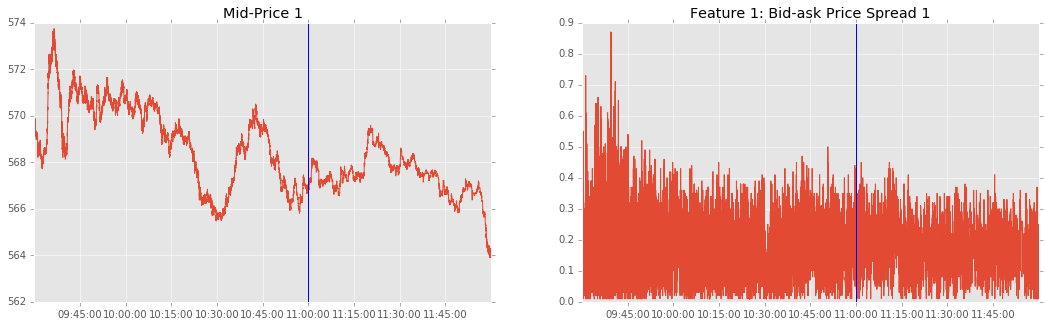
\includegraphics [width=0.9\linewidth,height=0.25\linewidth]{./figures/features_at11.png}
\caption{Feature behavior before and after 11:00AM}
\label{fig:fea_11}
\end{figure}
In future, to successfully implement the trading strategies from 11:00AM to 12:00PM, we probably need the data from 11:00 to 12:00 from yesterday or adding some time dummy variables.\\
Since none of the assumptions above are realistic, we would modify our strategies if assumptions were broken. If there was a transaction cost $x$ dollars for each transaction, we would modify our labeling for spread-crossings. For instance, we would define "Up" to be ($P_{t+\Delta t}^{bid} > P_t^{ask}+x$), and notice that $x$ could also be a percentage of the stock price. Also, if we were not limited by one stock per transaction, we would have to trade shares in a quantity subject to available best ask/ bid size, though we could trade at different price levels by pre-specifying a transaction volume. Lastly, if the fund were limited, we would have to devise a stop-loss mechanism to prevent huge losses due to misclassification.
\section{Discussion \& Conclusion}
For future analysis on the dynamic high-frequency trading strategies, we would concentrate more on the aspects that were not covered by this paper. Due to page limits and time constraints, we only looked at SVM with RBF kernel and random forest, yet did not try more advanced classification methods like Neural Network or gradient boosted decision trees, which could be great tools dealing with nonlinear feature space. Considering the computation power, we have narrowed our scope to the data in the limit order book in the data pre-processing part. With that being said, we were not able to use the advanced features $v_7-v_9$ in the message book, which might be important features in model fitting. Nevertheless, the original feature space was large enough to gain good accuracy.\\
Another limitation of the models was training the data from 9:30AM to 11:00AM, and implemented the strategies after 11:00AM without considering the time dependence of price movements. With enough computation power, the system should not only take one-day limit order book data. With multiple days data, we were able to inference on the data from 11AM to 12AM in other days. Overall, the computation power was not the main constraint for today's distributed system (like spark) used in real high-frequence trading, but it could be a serious problem to personal computors.\\
In conclusion, we have demonstrated the effectiveness of Support Vector Machines and Random Forests in classifying mid-price movements and spread-crossings. In particular, we have used one day data from limit order book to train models, and assessed the models based on a number of measures. Random Forest brought better model performance than SVM. Moreover, we have shown that a much smaller and efficient economized feature set could be used to attain the similar results compared to the entire feature space. In the end, we also tried to interprete the models, and implemented strategies to compute profit.

% the `Acknowledgments` section is required if you discussed the project
% with anyone else.

\bibliographystyle{plain}
\bibliography{finance}

\end{document}
